\documentclass[12pt]{UIdahoMastersThesis}
\makeatletter

\usepackage[latin1]{inputenc}
\makenoidxglossaries

%Preamble
\usepackage{tikz}
\usetikzlibrary{positioning}

\graphicspath{ {./img/} }

\usepackage[PetersLenny]{fncychap} %This makes the chapter titles fancy: If you don't want it fancy, delete this line and the chapter title formatting under the \frontmatter below
	\ChNameVar{\LARGE\scshape}
	\ChTitleVar{\Huge\scshape}

%Make post-it notes!
\usepackage[colorinlistoftodos,prependcaption,textsize=tiny]{todonotes}
\newcommandx{\note}[2][1=]{\todo[linecolor=orange,backgroundcolor=yellow!25,bordercolor=orange,#1]{#2}}

% --------------------------------------------------------------------------
% Thesis Information
\title{Design of a \acs{pid} Controller for a Molten Salt Microreactor}
\author{Sam J. Root}
\thesisdegree{Master of Science}
\major{Nuclear Engineering}
\advisor{Michael McKellar, Ph.D.}
\cmone{Dakota Roberson, Ph.D.}
\cmtwo{Robert A. Borrelli, Ph.D.}
\deptadmin{Indrajit Charit, Ph.D.}
\graddate{May, 2023}
% -------------------------------------------------------------------------

\linespread{1.3}%1.3 is on-and-a-half-spacing

% Defines section counter for front-matter. This way section number does not appear in the TOC for front-matter sections
\setcounter{secnumdepth}{0}

% Sets what level of sections show up in the table of contents. 0 = sections, 1 = subsections, 2 = sub-subsections, etc.
\setcounter{tocdepth}{1}


% Configure the PDF output (Most of this is optional, it just adds metadata to the PDF)
\usepackage[% pdftex
pdfauthor=Sam J. Root,
pdftitle=MsNB Control System,
pdfsubject={Controls},
pdfkeywords={Molten Salt Reactor;Molten Salt Nuclear Battery;Microreactor;Process Control},
pdfproducer={ShareLatex},  % e.g ShareLatex
pdfcreator={pdflatex},
pdfprintscaling={AppDefault}]{hyperref}

% Configure hyperlinks
\hypersetup{
	colorlinks=true, %set true if you want colored links
	linktoc=all,     %set to all if you want both sections and subsections linked
	linkcolor=black,  %choose some color if you want links to stand out
	citecolor=black,
	urlcolor=black,
}

% Changes default indenting in list of figures to 0
%\makeatletter
\renewcommand*\l@figure{\@dottedtocline{1}{0em}{2.3em}}% Default: 1.5em/2.3em
\let\l@table\l@figure
%\makeatother

% ------------------------------------------------------------
% ------------------------------------------------------------
% ------------------------------------------------------------
\begin{document}

\frontmatter

%\titleformat{\chapter}[block]{\scshape\LARGE}{\centering\chaptertitlename\  \thechapter:}{1ex}{\centering}{}\titlespacing{\chapter}{0pt}{-40pt}{20pt}

\titleformat{\section}[hang]{\scshape\Large}{\thesection}{1ex}{}
    \titlespacing{\section}{0pt}{0pt}{10pt}
	%\titlespacing*{\section}{0pt}{-50pt}{40pt}

\titleformat{\subsection}[hang]{\scshape\large}{\thesection}{1ex}{}
    \titlespacing{\subsection}{0pt}{0pt}{10pt}
	%\titlespacing*{\subsection}{0pt}{-50pt}{40pt}


% Head------------------------------------------------------------
% -- Title Page --
\thesistitlepage

% -- Abstract --
\frontmattersection{Abstract}
%Abstract
\begin{center}
	{\LARGE\textsc{Abstract}}
\end{center}

\lipsum[1-2]


% -- Acknowledgements --
 \frontmattersection{Acknowledgements}
\begin{center}
   {\LARGE\textsc{Acknowledgements}}

   This work and my coursework was completed under a Graduate Fellowship funded by \acf{nrc}. 



% -- Dedication --
 \frontmattersection{Dedication}
 \vspace*{\fill}
\begin{center}
{\LARGE\textsc{Dedication}}\vspace{0.5cm}

To my mother, Tammy, who planted and nurtured my love of science. To my father, Paul, who taught me how to design and build, and showed me that I am an engineer. To my cats, Babe and Bunyan, who stayed up with me all those late nights studying and writing. Thank you for your endless support.

\end{center}
\vspace{\fill}


% ------------------------------------------------------------
% -- Table of Contents --
\frontmattersection{Table of Contents}
\tableofcontents
\newpage

% -- List of Tables --
\frontmattersection{List of Tables}
\listoftables
\newpage

% -- List of Figures --
 \frontmattersection{List of Figures}
 \listoffigures
 \newpage

 % -- List of Codes --
 \frontmattersection{List of Codes}
 \listof{code}{List of Codes}
 \newpage

% -- List of Acronyms --
\frontmattersection{List of Acronyms}
\printnoidxglossary
\newpage

% ------------------------------------------------------------
\mainmatter  % Starts the content part of the thesis
\setcounter{secnumdepth}{1}  % Sets depth section numbers go to.
% NOTE !! : There is a bug currently where they will not work at depth of 3, e.g section 1.2.3 will not display, but 1.2 will.

% ------------------------------------------------------------
% -- Introduction --
\chapter{Introduction}
\label{Chapter:Introduction}

\section{Background}
The \acf{msnb} is a self contained design for a liquid fueled molten salt microreactor \cite{CarterPHD,PetersonMS}. It is fueled by an inorganic form of uranium, \UF, dissolved in a coolant salt such as \flinak (a eutectic mixture of three alkali fluorides) or \flibe  (a mixture of $LiF$ and $BeF_2$) \cite{RoperOverview}. Heat is generated in the core by fission, is transported by the natural circulation of the coolant/fuel salt, and rejected to a secondary working fluid in an integrated heat exchanger. Criticality is manipulated using axial control drums, which may be rotated to aim either a neutron reflecting material or a neutron absorbing material towards the core.

\subsection{Micro Reactors}
Its like a reactor but smol. This is a test from CAES.

\subsection{Molten Salt Reactors}
\acf{lwr}


\section{Scope}
As a developing design, work has been done on neutronics \cite{PetersonMS}, thermal-hydraulics and autonomous load following \cite{CarterPHD}, and corrosion concerns \cite{RoperPHD}. However, until now, little to no work has been done on the control system. First and foremost, this work details a multiphysics characterization of the \acs{msnb} required to design a feedback controller capable of matching the core power generation to the secondary power demand. In addition to the main control mode of following power transients during normal operation, specific discussion is centered around more dynamic time periods, namely: 
\begin{enumerate*}[label=\arabic*)]
    \item initial start-up;
    \item shutdown, both planned and emergency; and
    \item restart;
\end{enumerate*}

% -- Process Control Engineering --
\chapter{Process Control Engineering}
\label{Chapter:Controls}

\section{Feedback}

\section{Feedforward}
The term `Feedforward' can be used to refer to any element in the control block diagram that exists outside of the feedback loop.

\subsection{Disturbance Feedforward}
Not that useful since disturbance transport delay is on the order of minutes and disturbance dynamics are on the order of milliseconds

\subsection{Pre-Filter}
This could be electronic (less ideal) or physically realized by decoupling 


\section{Time Variance}
Fissile depletion - time function parameters or look-up table to gain-schedule and turn the time variant system into a shift invariant system.

In addition to the relatively slow time variance of fissile fuel depletion during steady-state critical operation, there are specific times in a \acs{msnb}'s expected operational life-cycle that exhibit a higher degree of time variance: 
\begin{enumerate*}
\item Start-up; \item Shut-down; and \item{Re-start}.
\end{enumerate*}

\subsection{Start-up}
Black-start may need to deal with thawing salt - main concern is fission product neutron poison build-up (discuss the burnable poison stuff)

\subsection{Shut-down}
Planned shut-down

Emergency Shutdown/SCRAM(must be passive)

Decay heat and keeping the salt liquid for restart

\subsection{Re-start}
\Xe stripper



% -- Reactor Characterization --
\chapter{Reactor Characterization}
\label{Chapter:Modeling}

\section{Reactor Design selection}

\section{Neutronics Modeling}

\section{Process Simulation}

% -- Controller Design --
\chapter{Controller Design}
\label{Chapter:Design}

\section{Reactor Transfer Function}

\section{Tuning Methodology}


% -- Reactor Characterization --
\chapter{Results and Analysis}
\label{Chapter:Results}

Tables and figures are handled well by \LaTeX . 

\section{Tables}

Tables can be generated using the tabular environment. To make it possible to reference them, include a caption, and automatically populate the list of tables, wrap this in the table environment.

\begin{table}[h!]
    \caption[Relevant Nuclear Constants]{Relevant nuclear constants \cite{Lamarsh}.}
    \centering\begin{tabular}{c|ccc}
                   & $\gamma \;(\%)$ & $\lambda \; (hr^{-1})$ & $\sigma \; (Mb)$ \\ \hline
        \I  & 6.39            & 0.1035                 & -                \\
        \Xe & 0.237           & 0.0753                 & 2.65
    \end{tabular}
    \label{params}
\end{table}

The caption contains two arguments. The first is wrapped in square brackets and is the "short" version that will populate in the List of Tables. The second is the "long" version, wrapped in curly braces, that will populate above the table. Table \ref{params} has 4 columns, each of which has centered data, with a vertical line after the first column. This is specified by the argument \verb={c|ccc}= after \verb=\begin{tabular}=. Columns are delimited by \& and rows are delimited by \verb=\\=. The label should come after \verb=\end{tabular}= so the compiler doesn't get confused.

\section{Figures}
The figure environment can be used to load in various images and other figures. Like with the table environment, you can develop a label to reference the figure in text, and both a short version and long version of the caption. This is handy to keep your List of Figures tidy while allowing for very descriptive captions under the figure.

\newpage

\subsection{Static Images}
These are included using the \verb=\includegraphics[options]{name}= command. There is a lot more information on the internet, including Dr. Trefor's videos. Figure \ref{BC} is an example. The argument after the \verb=\begin{figure}= is used to position the figure.

\begin{figure}[h!]
    \centering
    \includegraphics[width=0.25\textwidth]{BC}
    \caption[Big Chungus.]{A humorous image of an overweight Buggs Bunny, often referred to as `Big Chungus'.}
    \label{BC}
\end{figure}

\subsection{User Generated Drawings}

Tikz is a package that allows you to make very nice drawings right in \LaTeX \;. Dr. Trefor has a tutorial. The learning curve is steep, and honestly is more difficult to use than GUI sandbox based drawing application, but it has the benefit of being able to keep typeface formatting very consistent. See how nice the equations look in Figure \ref{strip}? Try doing that in MS Paint. 

\begin{figure}[h!]\centering
    

\begin{tikzpicture}
\draw[green, very thick] (-1,-1) rectangle (1,1);
\filldraw[green!10] (-1,-1) rectangle (1,1);
%Bottom
\draw[->] (0,-2)--(0,-1);
\draw node at (-0.15,-2.15) {\small{$c_{He}^{in} = 0$}};
%Top
\draw[->] (0,1)--(0,2);
\draw node at (0.15,2.15) {\small{$c_{He}^{out} = \nicefrac{c_{salt}^{out}}{H^*}$}};
%Left
\draw[->] (-2.75,0)--(-1,0);
\draw node at (-1.0,0.5) [anchor=east]{\small{$c_{salt}^{in} = Xe(t)$}} ;
%Right
\draw[->] (1,0)--(4,0);
\draw node at (1.0,0.5) [anchor = west]{\small{$c_{salt}^{out} = c_{salt}^{in}-c_{He}^{out}\frac{\dot{V}_{He}}{\dot{V}_{salt}}$}};
\end{tikzpicture}

    \caption{Schematic Drawing of Xenon Stripping Module} 
    \label{strip}
\end{figure}

\newpage
\subsection{Animations}
The graphicx package cannot accept .gif files, so the animate package can be used as a proxy. You will need each frame to be an individual .png, but this allows you to stack images over one another, which can give a time component to 2-D plots, or allow you to look at multiple planes of a drawing in a single figure. You will need to open the file in a proper PDF viewer like Adobe - web browsers and PDF previewers found in Overleaf, Atom, VSCode, etc. cannot handle this powerful functionality. I'm not sure if this functionality is allowed in the actual thesis submission, but it can be useful in presentations or meetings. Figure \ref{Bateman} is a visualization of the Bateman equations  causing the xenon spike following the shutdown of a nuclear reactor. It loops through bar-200 to bar-248 at 2 frames per second. You can also step through frame by frame using the arrow controls. Note that feature can cause compile times to be very long so you may wish to comment it out. 

\begin{figure}[h!]
    \centering
    \animategraphics[width=0.60\textwidth, controls]{2}{scram/bar-}{200}{248}
    \caption{Nuclide Concentration Rates of Change - Reactor Scram}
    \label{Bateman}
\end{figure}

% -- Reactor Characterization --
\chapter{Conclusions}
\label{Chapter:Conclusions}

\section{Limitations}

\section{Future Work}

\section{Summary Remarks}

% ------------------------------------------------------------
% -- References -- 

\clearpage
\renewcommand\bibname{References}
\addcontentsline{toc}{chapter}{\textsc{\bibname}}
\bibliographystyle{nsf}
\bibliography{References.bib}

% ------------------------------------------------------------
% -- Appendices --
\clearpage 
\appendix % Marks start of appendices

%Test
\chapter{Test}


\begin{code}\caption{Hello!} \begin{python}
    print("Hello World") #comment
    try:
        a=2/x
    except ZeroDivisionError:
        print('undefined')
\end{python}\label{code:hello}\end{code}

Inline codes like \pyth{import numpy}

\begin{code}\caption{F strings}
\inputpython{py/test.py}{1}{3}
\label{code:fstrings}\end{code}
\chapter{What}

Straight Cash Homie

\end{document}

% ** DO NOT PUT ANYTHING AFTER THE END OF THE DOCUMENT! **
